\documentclass{beamer}

\usepackage[T2A]{fontenc}
\usepackage[utf8]{inputenc}
\usepackage[russian]{babel}

\usepackage{graphicx}
\usepackage{amsmath}
\usepackage{listings}
\usepackage[center]{caption}
% \usepackage[usenames,dvipsnames]{xcolor}

\usetheme{Madrid}
\usecolortheme{seagull}

\lstset{
	commentstyle=\color{green!80},
    keywordstyle=\color{blue},
    stringstyle=\color{red},
	tabsize=4,
	basicstyle=\ttfamily
}

\begin{document}

\title[Теория графов] {Теория графов и её приложения}
\subtitle{Отчёт по проектному заданию}
\author[Козырев С., Куклин Д.] {Козырев~С.~А., Куклин~Д.~В.}
\institute[СПбГУ]
{
  Факультет прикладной математики --- процессов управления\\
  Санкт-Петербургский государственный университет
}
\date[\today]{\today}
\logo{
\includegraphics[height=1.5cm]{pics/uni-logo.png}}

\frame{\titlepage}

\section{Постановка задачи и методы решения}

\begin{frame}
\frametitle{Постановка задачи}
Требовалось:
\begin{enumerate}
\pause
\item построить граф дорог Российского города,
\pause
\item оценить удобство размещения зданий,
\pause
\item спланировать размещение зданий.
\end{enumerate}
\end{frame}

\begin{frame}
\frametitle{Что мы выбрали}
\begin{enumerate}
\item C++ \pause, так как
	\begin{itemize}
	\item большинство проектов написаны либо на C, либо на C++,
	\pause	
	\item среди остальных C++ является наиболее быстрым,
	\pause
	\item Python простой,
	\end{itemize}
\pause
\item \textit{libosmium},
\pause
\item Нижний Новгород.
\end{enumerate}
\end{frame}

\subsection{Построение графа дорог}

\begin{frame}
\frametitle{OSM Specification}
Спецификация \textit{OSM} определяет следующие структуры данных:
\begin{itemize}
\item \textit{Node} (узел),
\item \textit{Way} (путь),
\item \textit{Relation} (отношение).
\end{itemize}
\end{frame}

\begin{frame}
\frametitle{Извлечение карты}
\begin{figure}[ht]
	\centering	
	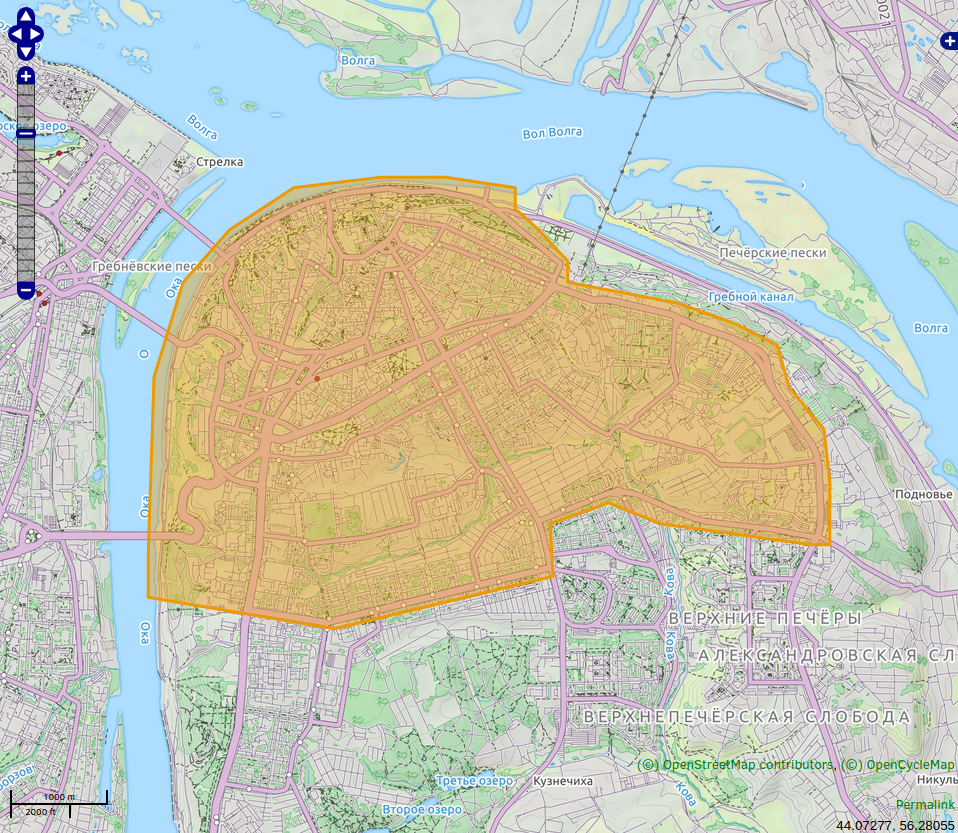
\includegraphics[width=0.4\textwidth]{pics/bbbike.png}
	\caption{Карта центра Нижнего Новгорода}
	\label{fig:bbbike}
	\end{figure}
\end{frame}

\begin{frame}[fragile]
\frametitle{Добавление путей}
\begin{lstlisting}[language=C++]
 unordered_map<uint64_t, bool> marked {};
 
void way(const Way& w) noexcept {
	if (!w.has_key("highway")) { return; }
	for (const auto& node: w.nodes()) {
		if (marked.contains(node)) {
			marked[node] |= true;
		} else {
			marked.insert({ node, false });
		}
	}
}
\end{lstlisting}
\end{frame}

\begin{frame}[fragile]
\frametitle{Добавление путей}
\begin{lstlisting}[language=C++]
for (const auto& curr: way.nodes()) {
	if (curr != first && curr != last) {
     	if (marked.at(curr)) {
     		auto d = ...; // One-way or two-way.
			auto w = haversine(pred, curr);
			routes.add_edge({ pred, curr }, w, d);
			pred = &curr;
		}
	}
}
\end{lstlisting}
\end{frame}

\begin{frame}
\frametitle{Расстояние между узлами}
Расстояние между двумя узлами можно вычислить, используя формулу гаверсинуса
\begin{gather*}
	\eta(\Theta) = \eta(\varphi_2 - \varphi_1) + \cos(\varphi_1) \cos(\varphi_2) \eta(\lambda_2 - \lambda_1), \\
	d = 2r \arcsin(\sqrt{\eta(\Theta)}),
\end{gather*}
	где $ \Theta $~--- центральный угол, $ \varphi_{1,2} $~--- широты в радианах, $ \lambda_{1,2} $~--- высоты в радианах и $ \eta(\theta) = \sin^2\left(\frac{\theta}{2}\right) $ для произвольного угла $ \theta $.
\end{frame}

\begin{frame}[fragile]
\frametitle{Структура \texttt{Node}}
\begin{lstlisting}[language=C++]
struct Node {
private:
	using Angle = long double; 
	
	uint64_t m_id = 0;
	Angle m_latitude = 0;
	Angle m_longitude = 0;
};
\end{lstlisting} 	
\end{frame}

\begin{frame}[fragile]
\frametitle{Структура \texttt{Graph}}
\begin{lstlisting}[language=C++]
struct Graph {
private:
	using Edge = pair<Node, Node>;
	using OutgoingEdges = unordered_map<Node, 
										Distance>;
	using AdjList = unordered_map<Node, 
								  OutgoingEdges>;
	
	AdjList m_data {};
};
\end{lstlisting}
\end{frame}

\begin{frame}
\frametitle{Структура \texttt{Building}}
Для каждого здания на карте
\begin{enumerate}
\item вычисляем барицентр здания,
\item находим ближайший к зданию узел дороги,
\item в структуре \textit{Building} связываем со зданием найденный узел.
\end{enumerate}
\end{frame}

\begin{frame}[fragile]
\frametitle{Структура \texttt{Building}}
\begin{lstlisting}[language=C++]
struct Building {
private:
	enum class Type {
		House,
		Facility
	};

	uint64_t m_id = 0;
	Type m_type;
	Angle m_latitude = 0;
	Angle m_longitude = 0;
	Node m_closest_node;
};
\end{lstlisting}
\end{frame}

\begin{frame}[fragile]
\frametitle{Структура \texttt{Map}}
\begin{lstlisting}[language=C++]
struct Map {
	struct Path {
	private:
		Building m_from, m_to;
		Distance m_distance;
	};

	struct TracedPath: public Path {
	private:
		vector<Node> m_trace;
	};
	
private:
	vector<Building> m_buildings;
	Graph m_graph;
};
\end{lstlisting}
\end{frame}

\begin{frame}
\frametitle{Проблема производительности}
Очевидно, карта составляется долго.\\
\textit{Libosmium} каждый раз производит чтение карты и заполнение структур.\\
Вопрос итоговой сложности является открытым, но любой желающий может получить на него ответ, изучив исходный код библиотеки.
\end{frame}

\begin{frame}[fragile]
\frametitle{Кэширование}
Мы обошли проблему, применив кэширование к структуре \texttt{Map}.\\
\begin{lstlisting}[language=C++]
template<typename T>
bool serialize(fs::path& filename, T&& data) {
	std::ofstream binary { filename };
	boost::binary_oarchive archive { binary };
	archive << data;
	binary.close();
	return true;
}
\end{lstlisting}
\end{frame}

\begin{frame}[fragile]
\frametitle{Кэширование}
\begin{lstlisting}[language=C++]
template<typename T>
bool deserialize(fs::path& filename, T&& data) {
	if (!fs::exists(filename)) { return false; }
	std::ifstream binary { filename };
	boost::binary_iarchive archive { binary };
	archive >> data;
	binary.close();
	return true;
}
\end{lstlisting}
\end{frame}

\end{document}